The proposed solution technique is designed to be implemented at the PCC(point of common coupling) of a microgrid containing distributed generation and energy storage. The objective is to optimize the use of energy storage under different pricing schemes taking advantage of DG and load forecasting. Figure \ref{fig:F1_CA} shows the top level architecture of the control strategy. As seen in the figure the BMS(battery management system) will optimize the power use from the DG plant, the utility grid and the ES. It will take in the RTP prediction, load prediction and PV prediction and generate optimum battery charge and discharge references based on the current and forecasted data.

\begin{figure}[!ht]
    \centering
    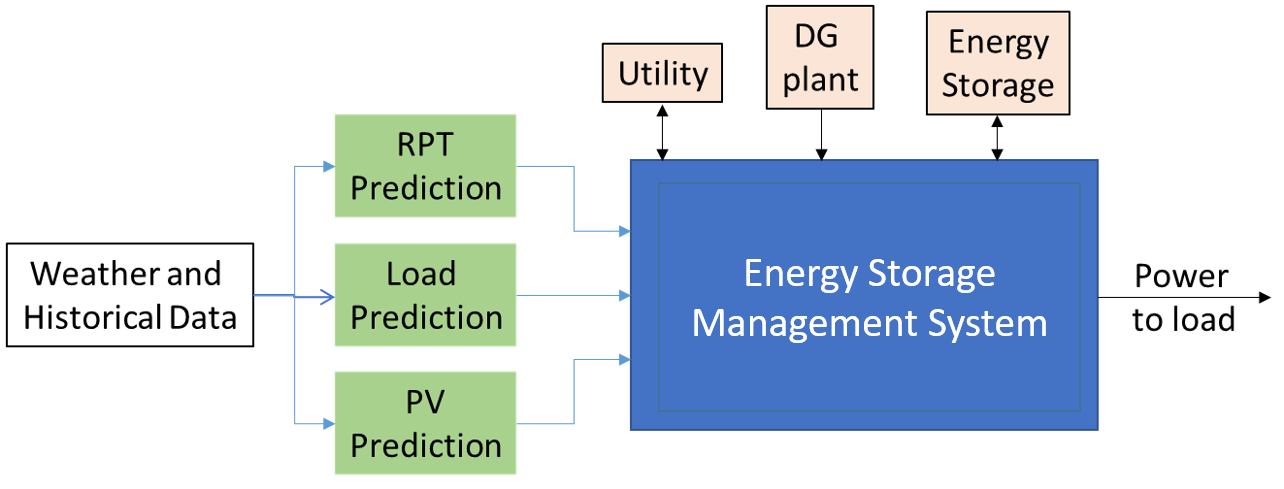
\includegraphics[width = \linewidth]{figs/EMS_FIG.png}
    \caption{Controller top level architecture}
    \label{fig:F1_CA}
\end{figure}

The solution has to take into account the current status of the system as well as the future forecasted state of the system to determine the most optimum time to charge and discharge the energy storage. To find the most cost optimum solution based on the current system status and future forecasts the optimization problem is formulated as a graph search problem. To represent the solution space of the problem as a graph the state of charge (SOC) of the ESS is discretized. Also the time until the prediction horizon is also represented in discrete steps. Figure \ref{fig:F1_Dis} represents a simple example of the discretized solution space.

\begin{figure}[!ht]
    \centering
    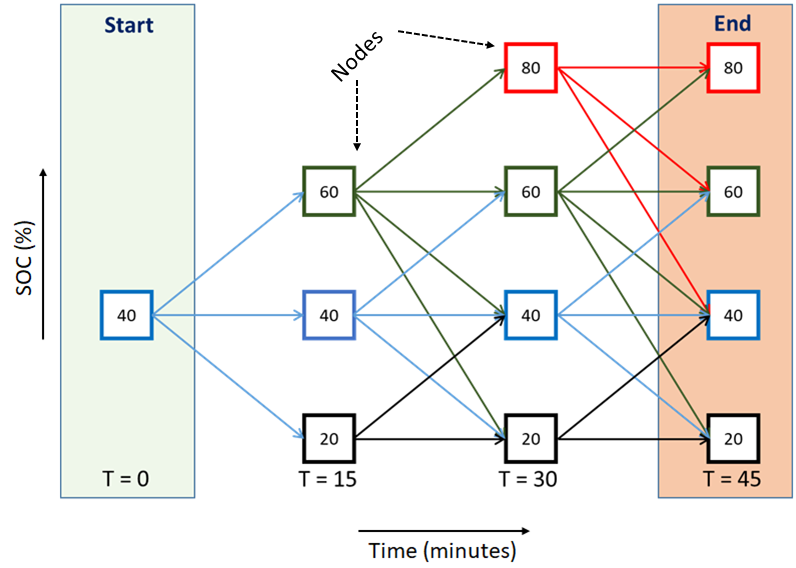
\includegraphics[width = \linewidth]{figs/F1_1_Dis.png}
    \caption{Discretizing solution space}
    \label{fig:F1_Dis}
\end{figure}
Here, the horizontal axis represents time and vertical axis represents discrete states of charge for the energy storage. In this scenario it is assumed that the algorithm recalculates the solution every 15 minutes based on available data. The SOC of the ESS is discretized in steps of 20\% and the SOC is limited between 80\% and 20\%. It is also assumed that the ESS can discharge a maximum of 40\% of it's maximum charge and charge a maximum of 20\% of it's charge in a 15 minute time step. Taking these features into consideration a directed graph is constructed in figure \ref{fig:F1_Dis}. The colored boxes represent nodes on the graph. The numbers inside the boxes represent the SOC of the ESS at that node. The arrows from the boxes represent all the possible states the ESS can be in in the next time step according to the constraints mentioned before. The arrows are treated as edges of the graph nodes. In this case the edges are unidirectional. The cost of the edges for a node at time $T = n$ are calculated using equation (\ref{eq:1}).
\begin{equation}
\label{eq:1}
    C_{EDGE} = C_{ESS}+C_{GRID}(n)
\end{equation}
Where,
$$
C_{ESS} = E_{ESS}*R_{ESS} 
$$
$$
E_{ESS} = (SOC_p - SOC_c)*ESS_{CAP}
$$
$$
C_{GRID}(n) = (P_{GRID}(n)*\Delta T + E_{ESS})*RTP(n)
$$

Here, $C_{EDGE}(n)$, $C_{ESS}(n)$ and $C_{GRID}(n)$ represent the cost of the Edge, cost of energy storage system and the cost of using the grid energy. $SOC_p and SOC_c$ are the states of charge of the parent and child node respectively. The parent node is the node the edge originates from and the child node is the node where the edge ends. $ESS_{CAP}$ is the total capacity of the energy storage. $R_{ESS}$ represent the \$/kwh cost of using the ESS. $P_{GRID}(n)$ is the power required from the grind at the $n^{th}$ time step. $\Delta T$ is the difference in time between the $n^{th}$ and $(n+1)^{th}$ time step. $RTP(n)$ represents the real time price of energy at the $n^{th}$ time step. 